{
\lstset{breakatwhitespace=true,breaklines=true}
\section{PDELab backends}
\label{sec:pdelab-backends}

\begin{frame}
  \frametitle<presentation>{PDELab backend}
  \begin{itemize}
  \item Linear algebra is decoupled from the discretization.
  \item Provides unique access interface for matrices, vectors and
    solvers.
  \item (Often) easily extensible for use of other libraries.
  \item Minimal knowledge of the underlying libraries required.
  \end{itemize}
\end{frame}

\begin{frame}
  \frametitle{PDELab backend in UML}
  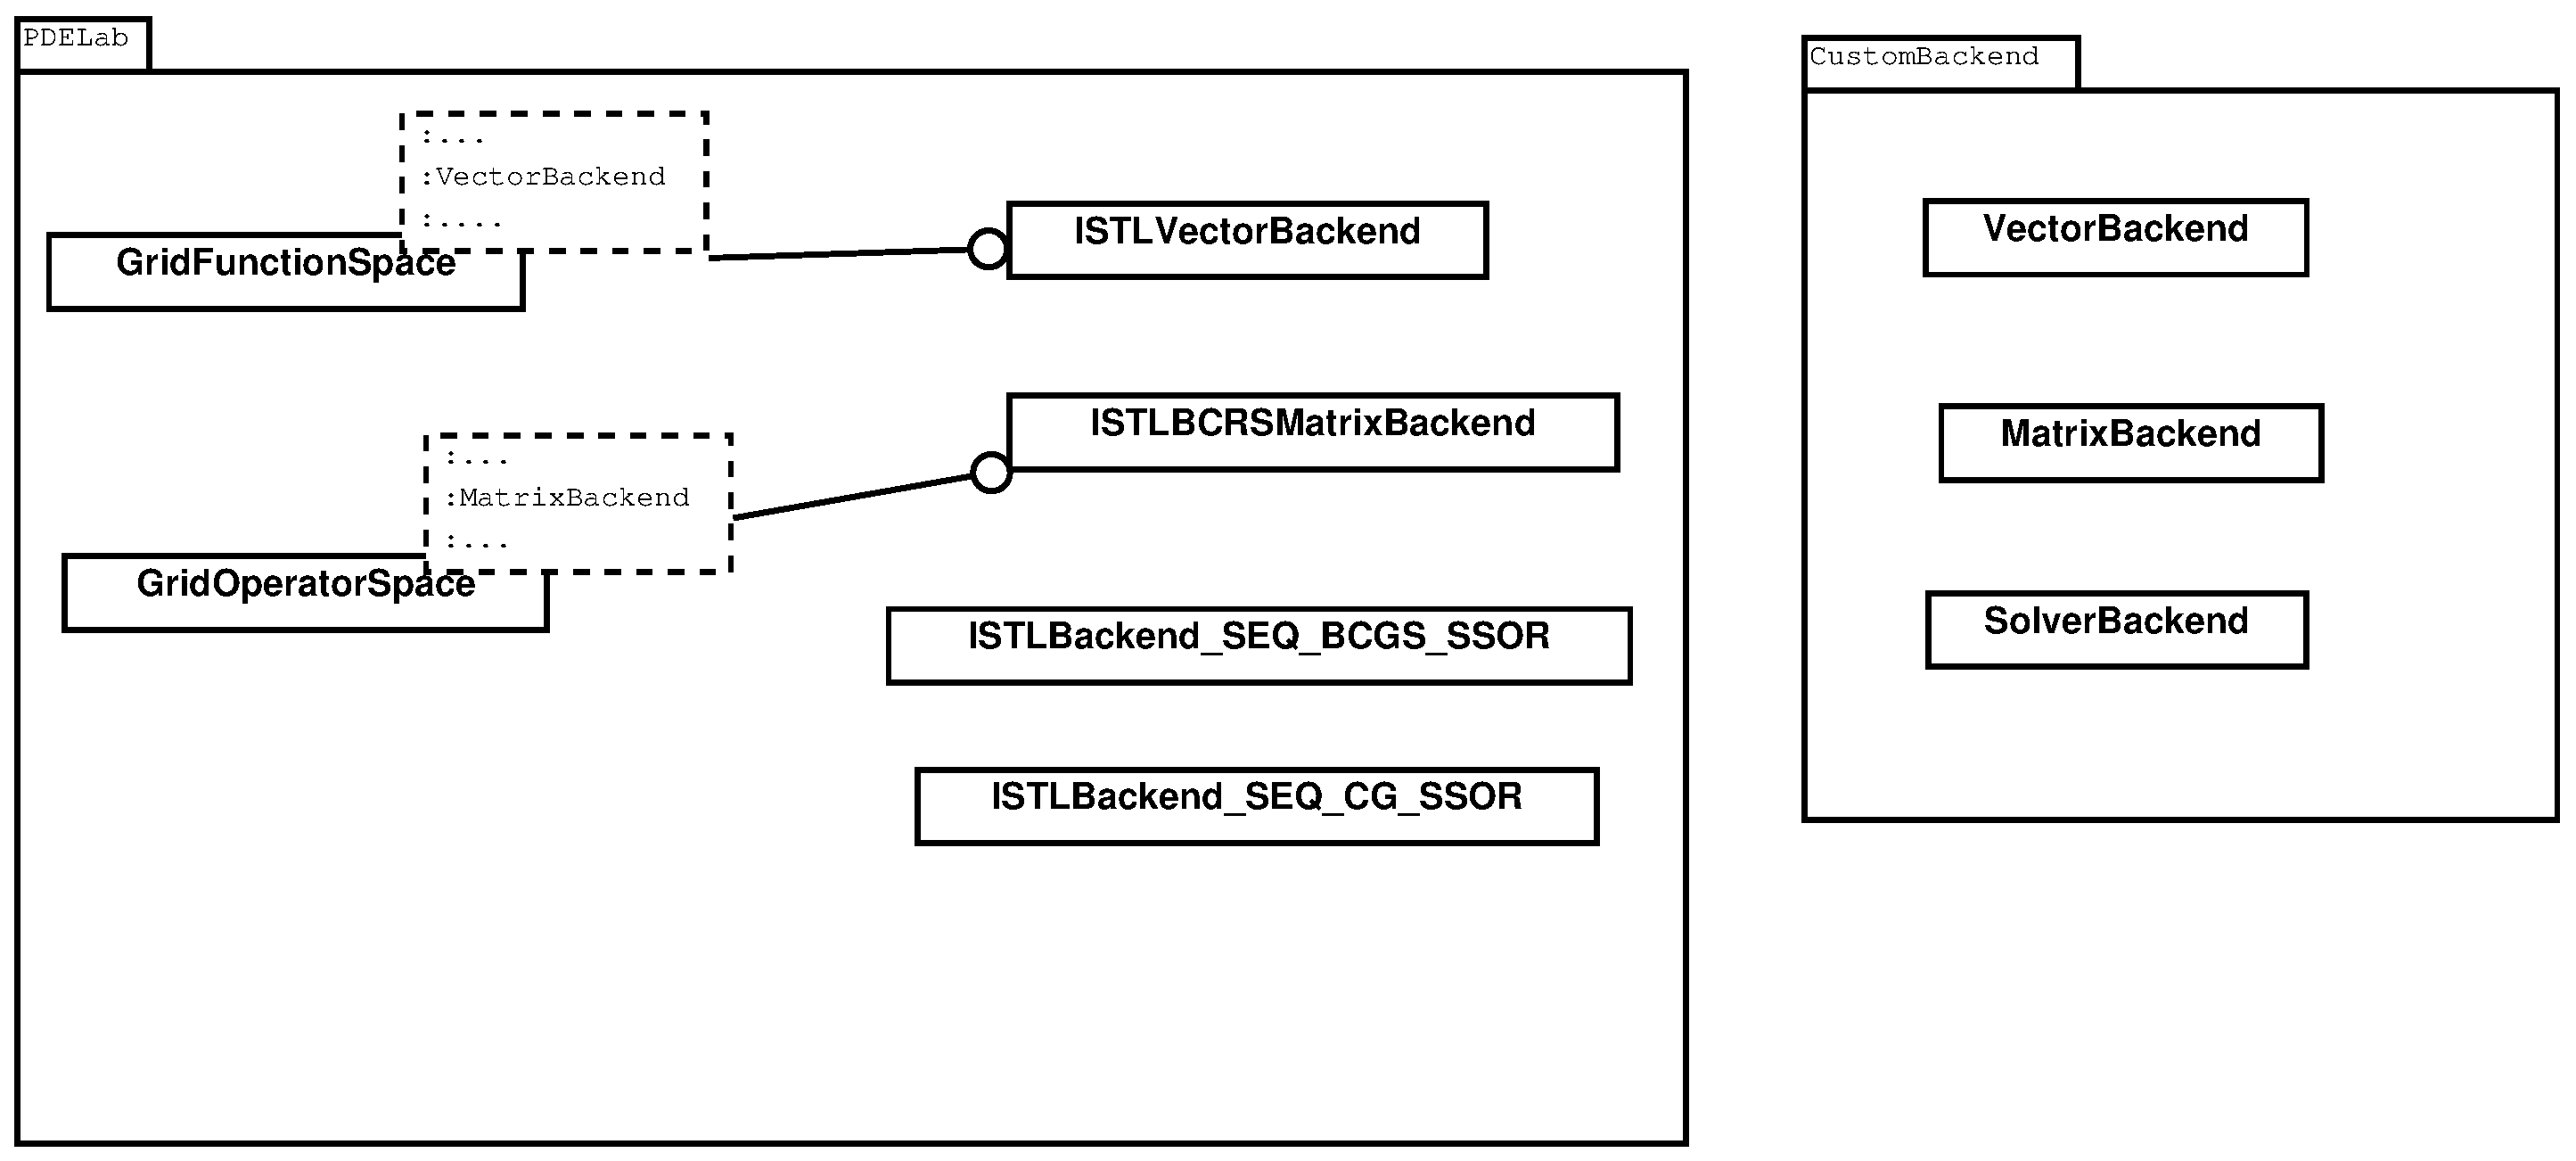
\includegraphics[width=\textwidth]{./EPS/backend}
\end{frame}
\subsection{Interface}
\label{sec:interface}

\subsubsection{The Vector Backend}
\label{sec:vector-backend}

\begin{frame}
  \frametitle<presentation>{The Vector Backend}
  \begin{itemize}
  \item It is a class not a namespace to allow template parameterization!
  \item Provides the actual container type as
    \lstinline!template<class T, class E> Vector!.
  \item Associated type \lstinline!size_type! used for index access.
  \item Const and mutable data access with 
    \lstinline!access(Vector<T,E>& cont, size_type i)!
  \end{itemize}
\end{frame}

\begin{frame}[fragile]
  \frametitle{Sample Vector Container}
  \begin{itemize}
  \item Template parameter T is the type of the grid function used.
  \item Template parameter E is the value type (e.g. double, float).
  \end{itemize}
  \begin{lstlisting}[basicstyle=\scriptsize]
    template<typename T, typename E>
    class VectorContainer 
    {
      public:
      // The stored element type
      typedef E ElementType;
      // The backend we are associated with
      typedef ISTLVectorBackend<BLOCKSIZE> Backend;
      
      //constructor with grid function space t
      VectorContainer (const T& t_);

      //constructor with grid function space t, initial value e
      VectorContainer (const T& t_, const E& e);
      
      // assignment
      VectorContainer& operator= (const E& e);
    };
  \end{lstlisting}
\end{frame}
\subsubsection{The Matrix Backend}
\label{sec:vector-backend}

\begin{frame}
  \frametitle<presentation>{The Matrix Backend}
  \begin{itemize}
  \item It is a class not a namespace to allow template
    parameterization!
  \item Provides the actual container type as
    \lstinline!template<class T, class E> Matrix!.
%  \item Provides associated type \lstinline!Pattern! for setting up
%    the sparsity pattern.
  \item Provides method \lstinline!clearRow(RI i, C& c)! for setting
    the values of row with index $i$ of container \lstinline!c! to zero.
  \end{itemize}
\end{frame}

\begin{frame}[fragile]
  \frametitle{The Matrix Container}
\begin{itemize}
  \item Template parameter T is the type of the grid function used.
  \item Template parameter E is the value type (e.g. double, float).
  \end{itemize}
  \begin{lstlisting}[basicstyle=\scriptsize]
template<class T, class E>
class MatrixContainer{
  public:
    // The stored element type
    typedef typename E ElementType;
    // The backend we are associated with
    typedef ISTLMatrixBackend<ROWBLOCKSIZE,COLBLOCKSIZE> Backend;
      
    //constructor with grid operator space t
    // Needs to setup the whole sparsity pattern.
    MatrixContainer (const T& t_);
      
    // assignment
    MatrixContainer& operator= (const E& e);
};
  \end{lstlisting}
\end{frame}
\begin{frame}[fragile]
  \frametitle{Sparse Matrix Setup in PDELab}
  \begin{itemize}
  \item Setting up a sparse matrix is a two step procedure:
    \begin{enumerate}
    \item Setting up the sparsity pattern.
    \item Filling the matrix with the values.
    \end{enumerate}
  \item First step is performed by the contructor of the matrix
    container.
  \item Second step is performed by the member function
    \lstinline!jacobian! of the grid operator space.
  \end{itemize}

\end{frame}

\subsubsection{The Linear Solver Backend}
\label{sec:line-solv-back}

\begin{frame}[fragile]
  \frametitle<presentation>{The Linear Solver Backend}
  \begin{itemize}
  \item Provides vector norm method needed by nonlinear PDELab solvers:
      \begin{lstlisting}
template<class V>
typename V::ElementType norm(const V& v) const;
      \end{lstlisting}
    \item Member function \lstinline!result()! returns statistics
      about the solution phase in an instance of the
      \lstinline!template<class T> LinearSolverResult! class template.
\item Use member function 
  \begin{lstlisting}
template<class M.class V,class W>
apply(M& A, V& z, W& r, typename V::ElementType reduction);
  \end{lstlisting}
  to (iteratively) solve $Az=r$ until the prescribed relative defect
  reduction is achieved.
  \item For ISTL it hides a lot of the compexity that heavy usage of
    templates imposes on the user.
  \end{itemize}
\end{frame}

\subsection{The Iterative Solver Template Library}
\label{sec:iter-solv-templ}

\subsubsection{Block Structure in FE Matrices}
\label{sec:motivation}
\begin{frame} \frametitle{PDE Systems}
  \begin{block}{}
      We have several unknowns and therefore several grid functions
      when dealing with PDE Systems.
      For the simple case that each function has the same structure we
      can use the following special ordering and blocking approaches:
  \begin{itemize}
  \item Equation-wise blocking: All degrees of freedom associated with
    the same unknown are blocked together.
  \item Point-wise blocking: All degrees of freedom associated with
    the same point (or element) are blocked together.
  \item No blocking is used.
  \end{itemize}
  \end{block}
  Currently the last two approaches are supported by PDELab with the
  ISTL backend.
\end{frame}
In the pictures below the degrees of freedom are visualized using
circles at the positions/entities they are associated with. Circles
with the same colour are blocked together. In the the entries in the
resulting matrix are dense and sparse matrices for the equation-wise
and point-wise blocking, respectively.
\begin{frame}
\frametitle{Some Examples for Block Structure}
\begin{block}{}
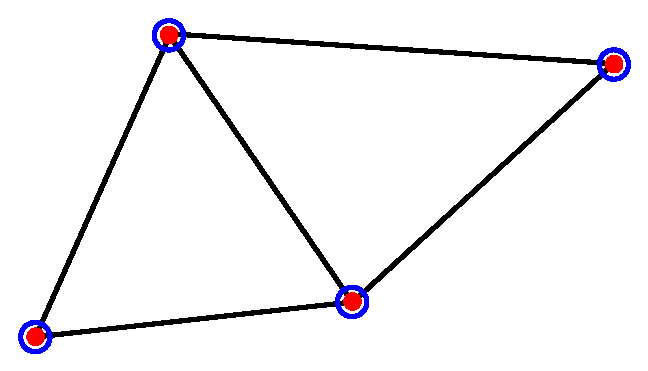
\includegraphics[width=0.48\textwidth]{./EPS/P1P1}\hfill
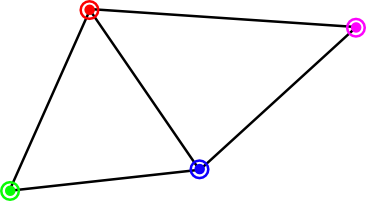
\includegraphics[width=0.48\textwidth]{./EPS/P1P1b}

\begin{minipage}{0.48\textwidth}
\centering $P_1\times P_1$ equation-wise
\end{minipage}
\begin{minipage}{0.48\textwidth}
\centering $P_1\times P_1$ point block
\end{minipage}

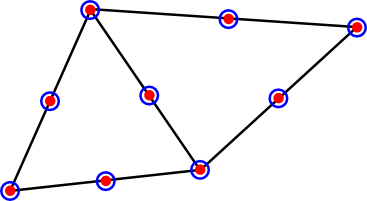
\includegraphics[width=0.48\textwidth]{./EPS/P2P2}\hfill
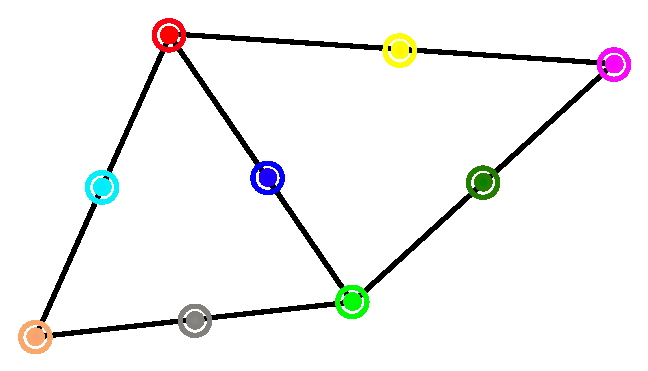
\includegraphics[width=0.48\textwidth]{./EPS/P2P2b}

\begin{minipage}{0.48\textwidth}
\centering $P_2\times P_2$ equation-wise
\end{minipage}
\begin{minipage}{0.48\textwidth}
\centering $P_2\times P_2$ point block
\end{minipage}
\end{block}
\end{frame}

\subsubsection{Matrix Vector Components}
\label{sec:matr-vect-comp}

\begin{frame}[fragile]
\frametitle{Block Structure in ISTL Matrices}
\begin{block}{}
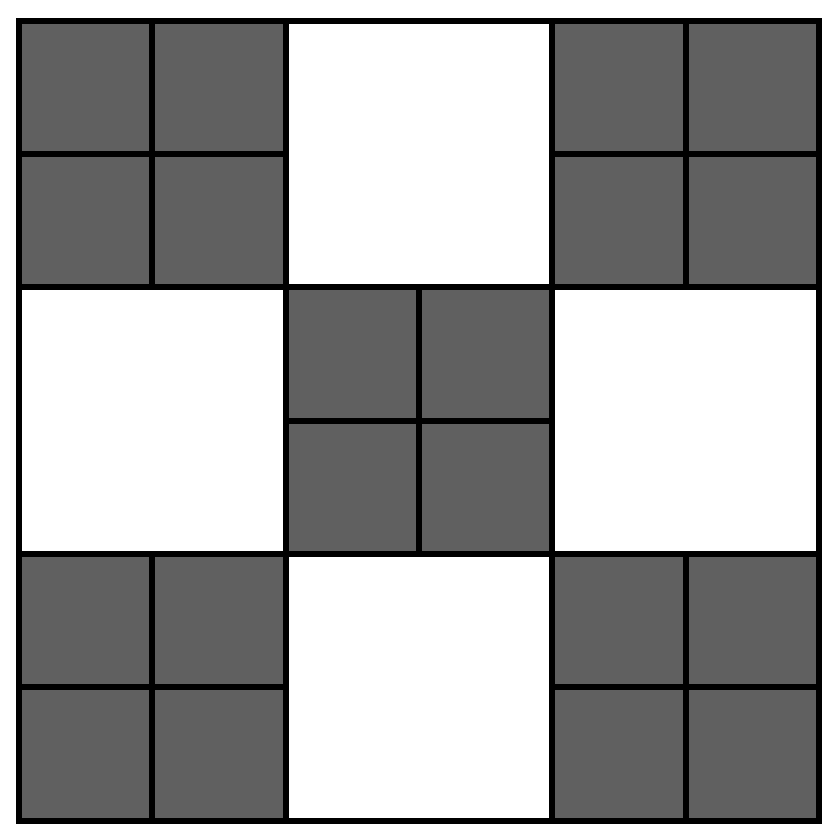
\includegraphics[width=0.3\textwidth]{./EPS/pointblockmatrix}\hfill
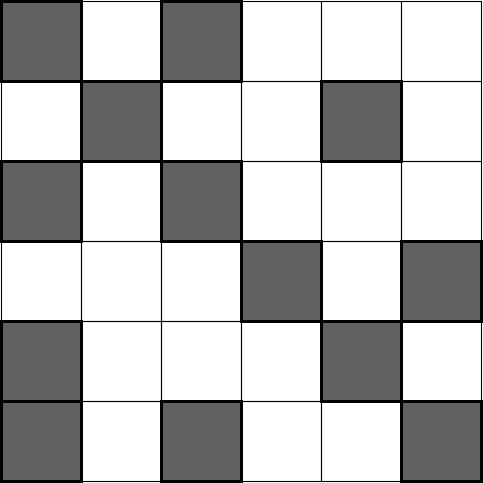
\includegraphics[width=0.3\textwidth]{./EPS/scalarmatrix}

\begin{minipage}{0.48\textwidth}
  \begin{itemize}
  \item  Point block matrix is a sparse matrix with small dense
blocks.
\item Realized by \lstinline!BCRSMatrix< FieldMatrix<E,2,2> >!. 
  \end{itemize}
\end{minipage}
\begin{minipage}{0.48\textwidth}
  \begin{itemize}
  \item Sparse matrix of scalars.
  \item Realized by \lstinline!BCRSMatrix< FieldMatrix<E,1,1> >!.
  \end{itemize}
\end{minipage}
\end{block}
\end{frame}


\subsubsection{The Backend}
\label{sec:backend}

\begin{frame}
  \frametitle{ISTL Vector Backend}
  \begin{itemize}
  \item \lstinline!template<int blocksize> class ISTLVectorBackend!
    is the currently available backend for ISTL vectors.
  \item The backend uses
    \lstinline!BlockVector<FieldVector<E,blocksize> >! as the
    underlying container.
  \item Attention: Make sure everything is correct for nonscalar backends
    \lstinline!blocksize!$>1$
  \end{itemize}
\end{frame}

\begin{frame}
  \frametitle{ISTL Matrix Backend}
  \begin{itemize} 
    \item \lstinline!template<int brows,int bcols> class ISTLBCRSMatrixBackend!
      is the currently available backend for ISTL sparse
      matrices.
    \item \lstinline!brows! is the number rows and \lstinline!bcols!
      is the number of columns of each matrix block.
  \item The backend uses
    \lstinline!BCRSMatrix<FieldMatrix<E,brows,bcols> >! as the
    underlying container.
  \item Attention: Make sure everything is correct for nonscalar backends
    \lstinline!blocksize!$>1$.
  \end{itemize}
\end{frame}
\begin{frame}[fragile]
  \frametitle{ISTL Sequential Solver Backends}
    \begin{itemize}
    \item \lstinline!ISTLBackend_SEQ_CG_SSOR!:  conjugate gradient method with SSOR preconditioner
    \item \lstinline!ISTLBackend_SEQ_BCGS_SSOR!: stabilized bi-conjugate gradient
      method with SSOR preconditioner
    \item \lstinline!ISTLBackend_SEQ_SuperLU!: SuperLU, a sparse
      direct solver
    \item \lstinline!template<class T> class ISTLBackend_SEQ_CG_AMG_SSOR! and
      \lstinline!template<class T> class ISTLBackend_SEQ_BICGS_AMG_SSOR! the
      above methods 
      preconditioned point-block AMG based on aggregation smoothed by SSOR.
    \end{itemize}
    Currently these sequential solvers are just a subset of the ones
  available in ISTL directly. More will follow in due time.
\end{frame}

\subsection{Parallel PDELab}
\label{sec:parallelization}

\begin{frame}
  \frametitle<presentatio>{Parallel PDELab}
  \begin{itemize}
  \item Go parallel by choosing
    \begin{enumerate}
    \item a suitable parallel grid (e.g. an overlapping one for
      overlapping domain decomposition methods),
    \item the correct constraints for the discretization of
      the PDE, and
    \item a suitable and matching parallel solver backend of the
      PDELab backend.
    \end{enumerate}
  \end{itemize}
\end{frame}

\begin{frame}
  \frametitle<presentation>{Parallel Solver Backends}
  
  There are three different kinds of parallel solvers classes
  available in the ISTL backend:
  \begin{itemize}
  \item Nonoverlapping domain decomposition
    methods.
  \item Overlapping domain decomposition metods.
  \item Data parallel solvers (e.g. AMG).
  \end{itemize}
\end{frame}

\begin{frame}
  \frametitle{Building Blocks for Parallel Solvers}

  \begin{itemize}
  \item The solvers in ISTL do not use matrix and vector structures
    directly,
  \item but implementations of \lstinline!Preconditioner!,
    \lstinline!LinearOperator! and \lstinline!ScalarProduct!.
  \item These components must match in the solver category
    (e.g. sequential, overlapping, nonoverlapping) and thus support
    the same data decomposition.
  \item Simply plugin parallel instances of the components to get
    parallel solvers.
  \end{itemize}
\end{frame}

\begin{frame}
  \frametitle<presentation>{Building Blocks for Parallel Solvers}
  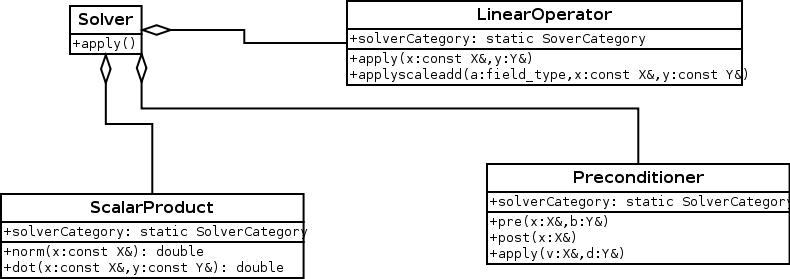
\includegraphics[width=\textwidth]{EPS/istlsolver}
\end{frame}

\begin{frame}
  \frametitle{Some Parallel Solver Backends}
  The solver backends can be found in header
  dune/pdelab/backend/istlsolverbackend.hh. Template parameter GFS is
  the type of the grid function space, template parameter C the type
  of the parallel constraints used.
  \begin{itemize}
  \item \lstinline!template<class GFS> class ISTLBackend_NOVLP_BCGS_NOPREC!:
    parallel unpreconditioned
    stabilized bi-conjugate gradient method for nonoverlapping grids.
    \item \lstinline!template<class GFS> class ISTLBackend_OVLP_BCGS_SSORk!:
      the above preconditioned with $k$ steps of SSOR.
    \item \lstinline!template<class GFS, class C> class ISTLBackend_OVLP_BCGS_SuperLU!:
      the first method preconditioned by an overlapping domain
      decomposition method with SuperLU for the problems local to the
      processors.
      \item \lstinline!template<class GFS> ISTLBackend_BCGS_AMG_SSOR!:
        the first method preconsitioned by parallel AMG smoothed by
        SSOR. Requires an overlapping grid!
  \end{itemize}
\end{frame}

\begin{frame}[fragile]
  \frametitle{Nonoverlapping example}
  \begin{lstlisting}[basicstyle=\tiny]
// 1. Create an non-overlapping grid
Dune::FieldVector<double,2> L(1.0);
Dune::FieldVector<int,2> N(16);
Dune::FieldVector<bool,2> periodic(false);
int overlap=0; // needs overlap 0 because overlap elements are not assembled
Dune::YaspGrid<2> grid(helper.getCommunicator(),L,N,periodic,overlap);
typedef Dune::YaspGrid<2>::LeafGridView GV;
const GV& gv=grid.leafView();

// 2. Create correctly constrained grid function space
typedef Dune::PDELab::Q1LocalFiniteElementMap<Coord,Real,dim> FEM;
FEM fem;
typedef Dune::PDELab::NonoverlappingConformingDirichletConstraints CON;
CON con;
typedef Dune::PDELab::ISTLVectorBackend<1> VBE;
typedef Dune::PDELab::GridFunctionSpace<GV,FEM,CON,VBE,
Dune::PDELab::SimpleGridFunctionStaticSize> GFS;
GFS gfs(gv,fem,con);
con.compute_ghosts(gfs); // con stores indices of ghost dofs
typedef ConvectionDiffusionProblem<GV,Real> Param;
Param param;
typedef Dune::PDELab::BoundaryConditionType_CD<Param> B;
B b(gv,param);
typedef Dune::PDELab::DirichletBoundaryCondition_CD<Param> G;
G g(gv,param);
\end{lstlisting}
\end{frame}
\begin{frame}[fragile]
\frametitle<presentation>{Nonoverlapping Example Continued}
  \begin{lstlisting}[basicstyle=\tiny]
// Compute constrained space
typedef typename GFS::template ConstraintsContainer<Real>::Type C;
C cg;
Dune::PDELab::constraints(b,gfs,cg);

// Compute affine shift
typedef typename GFS::template VectorContainer<Real>::Type V;
V x(gfs,0.0);
Dune::PDELab::interpolate(g,gfs,x);
Dune::PDELab::set_nonconstrained_dofs(cg,0.0,x);

// Make grid operator space
typedef Dune::PDELab::ConvectionDiffusion<Param> LOP; 
LOP lop(param,2);
typedef Dune::PDELab::ISTLBCRSMatrixBackend<1,1> MBE;
typedef Dune::PDELab::GridOperatorSpace<GFS,GFS,LOP,C,C,MBE,true> GOS;
GOS gos(gfs,cg,gfs,cg,lop);

// 3. Choose a linear solver 
typedef Dune::PDELab::ISTLBackend_NOVLP_BCGS_NOPREC<GFS> LS;
LS ls(gfs,5000,1);
...
\end{lstlisting}
  
\end{frame}

\begin{frame}[fragile]
  \frametitle{Overlapping Example}
  \begin{lstlisting}[basicstyle=\tiny]
// 1. Create an overlapping grid
Dune::FieldVector<double,2> L(1.0);
Dune::FieldVector<int,2> N(16);
Dune::FieldVector<bool,2> periodic(false);
int overlap=2; 
Dune::YaspGrid<2> grid(helper.getCommunicator(),L,N,periodic,overlap);
typedef Dune::YaspGrid<2>::LeafGridView GV;
const GV& gv=grid.leafView();

// 2. Create correctly constrained grid function space
typedef Dune::PDELab::Q1LocalFiniteElementMap<Coord,Real,dim> FEM;
FEM fem;
typedef Dune::PDELab::OverlappingConformingDirichletConstraints CON;
typedef Dune::PDELab::ISTLVectorBackend<1> VBE;
typedef Dune::PDELab::GridFunctionSpace<GV,FEM,CON,VBE,
Dune::PDELab::SimpleGridFunctionStaticSize> GFS;
GFS gfs(gv,fem);

//  define problem parameters
typedef ConvectionDiffusionProblem<GV,Real> Param;
Param param;
typedef Dune::PDELab::BoundaryConditionType_CD<Param> B;
B b(gv,param);
typedef Dune::PDELab::DirichletBoundaryCondition_CD<Param> G;
G g(gv,param);
\end{lstlisting}  
\end{frame}
\begin{frame}[fragile]
\frametitle<presentation>{Overlapping Example Continued}
  \begin{lstlisting}[basicstyle=\tiny]

//  Compute constrained space
typedef typename GFS::template ConstraintsContainer<Real>::Type C;
C cg;
Dune::PDELab::constraints(b,gfs,cg);
//  Compute affine shift
typedef typename GFS::template VectorContainer<Real>::Type V;
V x(gfs,0.0);
Dune::PDELab::interpolate(g,gfs,x);
Dune::PDELab::set_nonconstrained_dofs(cg,0.0,x);
// Make grid operator space
typedef Dune::PDELab::ConvectionDiffusion<Param> LOP; 
LOP lop(param,2);
typedef Dune::PDELab::ISTLBCRSMatrixBackend<1,1> MBE;
typedef Dune::PDELab::GridOperatorSpace<GFS,GFS,LOP,C,C,MBE> GOS;
GOS gos(gfs,cg,gfs,cg,lop);

// 3. Choose a linear solver 
typedef Dune::PDELab::ISTLBackend_OVLP_BCGS_SuperLU<GFS,C> LS;
LS ls(gfs,cg,5000,2);
...
\end{lstlisting}
  
\end{frame}
}
%%% Local Variables: 
%%% mode: latex
%%% TeX-master: 
%%% End: 
